%!TEX root = maze.tex
%!TEX program = lualatex
%!TEX encoding = utf-8
%!TEX spellcheck = en_US

\documentclass{easychair}
% !TeX root = design.tex
%!TEX program = lualatex


\usepackage[utf8]{inputenc}
\usepackage[T1]{fontenc}

\usepackage{fontspec}
\usepackage{lmodern}

% add page number
% \pagestyle{headings}

% beamer setting
% \usetheme{CambridgeUS}
% \setbeamertemplate{footline}[page number]
% \setbeamertemplate{blocks}[rounded][shadow=true]

% \pdfoptionpdfminorversion=7
% \pdfminorversion=6

% use table of content for each chapter
% \usepackage{minitoc}

% \usepackage[a-3u]{pdfx}

% \usepackage[toc,page]{appendix}
\usepackage[titletoc]{appendix}

% csquotes
\usepackage{csquotes}

% use biblatex
\usepackage[sorting=anyt,sortcites=true,backend=biber,url=false,doi=false,maxnames=7,isbn=false,firstinits=true,style=numeric]{biblatex}
% \addbibresource{reference}
\bibliography{reference}


% encoding (just for pdflatex)
% \usepackage[latin1]{inputenc}

% hyphenating
\usepackage[english]{babel}
% \usepackage[autostyle]{csquotes}

% AMS Math
\usepackage{braket}
% \usepackage{amsmath,amssymb,amsthm,mathtools}
% \usepackage{breqn}
\usepackage{amsmath,amssymb,mathtools,amsthm}
% \usepackage{unicode-math}
% \usepackage{lualatex-math}
% \usepackage{stix}
% \usepackage{cmbright}
% \usepackage{lmodern}
% \usepackage{lxfonts}
\usepackage{nicefrac}
\usepackage{stmaryrd}
\usepackage{xfrac}
% \usepackage{MnSymbol}


% for algorithm
%\usepackage{algorithm}
%\usepackage{algpseudocode}
\usepackage{algorithm2e}
\SetAlFnt{\small}

% hyperref
\usepackage{hyperref}
% \usepackage[pdfa]{tulhypref}
\hypersetup
{
%   bookmarks       = true,
  unicode         = true,
  pdftitle        = Maze challenge,
  pdfauthor       = Verimag, %auteur du document
  pdfsubject      = Maze challenge,
  pdftoolbar      = true, %barre d'outils non visible
  pdfmenubar      = true, %barre de menu visible
  pdfhighlight    = /O, %effet d'un clic sur un lien hypertexte
  colorlinks      = true, %couleurs sur les liens hypertextes
%   pdfpagemode = None, %aucun mode de page
%   pdfpagelayout = SinglePage, %ouverture en simple page
  pdffitwindow    = true, %pages ouvertes entierement dans toute la fenetre
  linkcolor       = violet, %couleur des liens hypertextes internes
  citecolor       = blue, %couleur des liens pour les citations
  urlcolor        = orange, %couleur des liens pour les url
%   pagebackref=true
%   bookmarksdepth  = 3
}

% \usepackage[sc]{mathpazo}
% \newfontfamily\DejaSans{DejaVu Sans}

\usepackage[usenames,dvipsnames,svgnames,table]{xcolor}
\definecolor{darkgoldenrod}{rgb}{0.72, 0.53, 0.04}
\definecolor{darkorchid}{rgb}{0.6, 0.2, 0.8}
% for listings
\usepackage{listings}
\lstset{basicstyle=\footnotesize\ttfamily,showspaces=false,frame=tb}
% \ltset{basicstyle=\small\ttfamily,showspaces=false,frame=tb}
\lstloadlanguages{C++,[x86masm]Assembler}

% graphicx and caption
\usepackage{graphicx}
% \usepackage{bmpsize}
% \usepackage[font={small}]{caption}
\usepackage{caption}
% \usepackage{subfig}
% \usepackage[config,position=t]{subfig}
\usepackage{subcaption}
% \captionsetup{compatibility=false}
% \DeclareCaptionLabelSeparator{periodspace}{.\quad}
% \captionsetup{font=footnotesize,labelsep=periodspace,singlelinecheck=false}
% \captionsetup[sub]{font=footnotesize,singlelinecheck=true}
% \renewcommand\thesubfigure{(\alph{subfigure})}
% \usepackage{rotating}
\usepackage{pdfpages}

% for smarter reference
\usepackage{cleveref}

% reference depth
\setcounter{secnumdepth}{2}

% for appendix
% \usepackage{appendix}

% for footnote
\usepackage{fancyvrb}
\VerbatimFootnotes

% for diagram
\usepackage{tikz}
\usetikzlibrary{calc,
                automata,
                arrows,
                matrix, 
                plotmarks,
                positioning,
                shapes,
                shapes.multipart,
                shapes.misc,
                decorations, 
                decorations.markings, 
                decorations.pathreplacing, 
                decorations.pathmorphing,
                backgrounds,
                fit,
                patterns}
% \usepackage{tkz-base}

% for commutative diagram
\usepackage{tikz-cd}
%\tikzset{commutative diagram/row}

\usepackage{wrapfig}

% for margin note
\usepackage{marginnote}

% for itemize
\usepackage{enumerate}
\usepackage[inline]{enumitem}
% \setitemize{label=\usebeamerfont*{itemize item}%
%   \usebeamercolor[fg]{itemize item}
%   \usebeamertemplate{itemize item}}

% create procedure environment
%\newtheorem{procedure}{Procedure}

% some tikz styles
% \tikzset{morphism/.style={circle,draw,thick,align=center,inner sep=0pt,minimum size=12pt}}
% \tikzset{bigmorphism/.style={circle,draw,thick,align=center,inner sep=0pt,minimum size=25pt}}
%\tikzset{objects/.style=}

% enumitem
% \usepackage{enumitem}

\usepackage{fancyvrb}

\usepackage{cprotect}

\usepackage{footmisc}

\usepackage{array}

% \usepackage{gnuplottex}

\usepackage{float}

\usepackage{mathrsfs}

\usepackage[export]{adjustbox}

\usepackage{rotating}

% for footnote
\usepackage{perpage} 
\MakePerPage{footnote}

\usepackage{parcolumns}

\usepackage{url}

% \usepackage{savetrees}

% \usepackage{floatrow}
% \floatsetup[table]{font=small}

% \newtheorem{principle}{Principle}
% \crefname{principle}{principle}{principles}
% \Crefname{principle}{Principle}{Principles}

\theoremstyle{plain}

% \newtheorem{hypothesis}{Hypothesis}
% \crefname{hypothesis}{hypothesis}{hypotheses}
% \Crefname{hypothesis}{Hypothesis}{Hypotheses}
% 
% \newtheorem{assumption}{Assumption}
% \crefname{assumption}{assumption}{assumptions}
% \Crefname{assumption}{Assumption}{Assumptions}
% 
% \newtheorem{heuristic}{Heuristic}
% \crefname{heuristic}{heuristic}{heuristics}
% \Crefname{heuristic}{Heuristic}{Heuristics}


\newtheorem{theorem}{Theorem}
\crefname{theorem}{theorem}{theorem}
\Crefname{theorem}{Theorem}{Theorems}

% \newtheorem{proposition}{Proposition}[section]
\newtheorem{proposition}{Proposition}
\crefname{proposition}{proposition}{propositions}
\Crefname{proposition}{Proposition}{Propositions}
% 
\newtheorem{corollary}{Corollary}[section]
\crefname{corollary}{corollary}{corollaries}
\Crefname{corollary}{Corollary}{Corollaries}

\newtheorem{problem}{Problem}
\crefname{problem}{problem}{problems}
\Crefname{problem}{Problem}{Problems}

\newtheorem{lemma}{Lemma}[section]
\crefname{lemma}{lemma}{lemmas}
\Crefname{lemma}{Lemma}{Lemmas}

\newtheorem{observation}{Observation}[section]
\crefname{observation}{observation}{observations}
\Crefname{observation}{Observation}{Observations}

\theoremstyle{definition}
% 
\newtheorem{definition}{Definition}[section]
\crefname{definition}{definition}{definitions}
\Crefname{definition}{Definition}{Definitions}
% 
\newtheorem{hypothesis}{Hypothesis}
\crefname{hypothesis}{hypothesis}{hypotheses}
\Crefname{hypothesis}{Hypothesis}{Hypotheses}

% \newtheoremstyle{dotlessP}{}{}{}{}{\color{blue}\bfseries}{}{ }{}

% \theoremstyle{dotlessP}
% \theoremstyle{plain}
\theoremstyle{remark}

% \newtheorem{example}{Example}[section]
\newtheorem{example}{Example}
\crefname{example}{example}{examples}
\Crefname{example}{Example}{Examples}

\theoremstyle{remark}

% \newtheorem{remark}{Remark}[section]
\newtheorem{remark}{Remark}
\crefname{remark}{remark}{remarks}
\Crefname{remark}{Remark}{Remarks}

\newtheorem{note}{Note}[section]
\crefname{note}{note}{notes}
\Crefname{note}{Note}{Notes}

\crefname{secinapp}{appendix}{appendices}
\Crefname{secinapp}{Appendix}{Appendices}

% \crefname{appendix}{appendix}{appendices}
% \Crefname{appendix}{Appendix}{Appendices}
% \newtheorem{corollary}{Corollary}

% \newtheoremstyle{dotlessP}{}{}{}{}{\color{blue}\bfseries}{}{ }{}
% \theoremstyle{dotlessP}

%%%% BINARY INSTRUCTION %%%%
% \newcommand{\jump}{{\tt jump}\xspace}
% \newcommand{\call}{{\tt call}\xspace}
% \newcommand{\ret}{{\tt ret}\xspace}
% \newcommand{\jcc}{{\tt jcc}\xspace}
% \newcommand{\instr}{{\tt i}\xspace}
% \newcommand{\code}{{\tt c}\xspace}
% 
% %%%% GENERAL %%%%%%%%%%
% \newcommand{\dcfg}[1]{{\cal G}_{#1}}
% \newcommand{\E}{{\cal E}}
% \newcommand{\V}{{\cal V}}
% % \newcommand{\T}{{\cal T}}
% \newcommand{\N}{{\mathbb{N}}}

% \newtheorem{problem}{Problem}
% \crefname{problem}{problem}{problems}
% \Crefname(problem}{Problem}{Problems}

% \makeatletter
% \let\@twosidetrue\@twosidefalse
% \let\@mparswitchtrue\@mparswitchfalse
% \makeatother

% \usepackage[left=0.5cm,right=0.5cm,top=0.5cm,bottom=0.5cm]{geometry}

% \vspace{-2.5mm}
% \setlength{\textfloatsep}{\baselineskip plus 0.2\baselineskip minus 0.2\baselineskip}
% \setlength{\textfloatsep}{10pt}
% \setlength{\belowcaptionskip}{-10pt}
% \setlength{\intextsep}{10pt}
% \setlength\abovedisplayskip{0pt}
% \usepackage[font=small,skip=10pt]{caption}
\allowdisplaybreaks

% \usepackage{titlesec}
% \titlespacing\section{0pt}{12pt plus 4pt minus 2pt}{0pt plus 2pt minus 2pt}

% \setlength{\parindent}{0pt}
% \usepackage[nodisplayskipstretch]{setspace}
% \setstretch{1.5}

% \definecolor{cornflowerblue}{rgb}{0.39, 0.58, 0.93}

% \usepackage{lmodern}
% \usepackage[sc]{mathpazo}
% \linespread{1.05}
% \usepackage{baskervald}
% \usepackage{nbaskerv}
% \usepackage[utf8]{inputenc}
% \usepackage[T1]{fontenc}
% \usepackage{luatextra}
% \defaultfontfeatures{Ligatures=TeX}

% \usepackage{unicode-math}
% \usepackage{lualatex-math}
% \usepackage{charter}
% \usepackage[expert]{mathdesign}

\usepackage{afterpage}
\usepackage{changepage}

\usepackage{minted}
\usemintedstyle{friendly}
\usepackage{tcolorbox}
\usepackage{etoolbox}
% \BeforeBeginEnvironment{minted}{\begin{tcolorbox}}%
% \AfterEndEnvironment{minted}{\end{tcolorbox}}%

% \setcounter{totalnumber}{1}
% \setcounter{topnumber}{1}
% \setcounter{bottomnumber}{1}
% \renewcommand{\topfraction}{.99}
% \renewcommand{\bottomfraction}{.99}
% \renewcommand{\textfraction}{.01}

% \makeatletter
% \newcommand*{\twopagepicture}[4]{%
%     \checkoddpage
%     \ifoddpage
%         \expandafter\@firstofone
%     \else
%         \expandafter\afterpage
%     \fi
%     {\afterpage{%
%     \if #1t%
%         \if #2p%
%             \thispagestyle{empty}%
%             \afterpage{\thispagestyle{empty}}%
%         \fi
%     \fi
%     \begin{figure}[#1]
%         \if #2p%
%             \if #1t%
%                 \vspace*{-\dimexpr1in+\voffset+\topmargin+\headheight+\headsep\relax}%
%             \fi
%         \fi
%         \if #1b%
%             \caption{#4}%
%         \fi
%         \makebox[\textwidth][l]{%
%         \if #2p\relax
%             \let\mywidth\paperwidth
%             \hskip-\dimexpr1in+\hoffset+\evensidemargin\relax
%         \else
%             \let\mywidth\linewidth
%         \fi
%         \adjustbox{trim=0 0 {.5\width} 0,clip}{\includegraphics[width=2\mywidth]{#3}}}%
%         \if #1b\else
%             \caption{#4}%
%         \fi
%         \if #2p%
%             \if #1b%
%                 \vspace*{-\dimexpr\paperheight-\textheight-1in-\voffset-\topmargin-\headheight-\headsep\relax}%
%             \fi
%         \fi
%     \end{figure}%
%     \begin{figure}[#1]
%         \if #2p%
%             \if #1t%
%                 \vspace*{-\dimexpr1in+\voffset+\topmargin+\headheight+\headsep\relax}%
%             \fi
%         \fi
%         \makebox[\textwidth][l]{%
%         \if #2p%
%             \let\mywidth\paperwidth
%             \hskip-\dimexpr1in+\hoffset+\oddsidemargin\relax
%         \else
%             \let\mywidth\linewidth
%         \fi
%         \adjustbox{trim={.5\width} 0 0 0,clip}{\includegraphics[width=2\mywidth]{#3}}}%
%         \if #2p%
%             \if #1b%
%                 \vspace*{-\dimexpr\paperheight-\textheight-1in-\voffset-\topmargin-\headheight-\headsep\relax}%
%             \fi
%         \fi
%     \end{figure}%
%     }}%
% }
% \makeatother

% \usepackage[usenames]{color}

% some tikz styles
\tikzset{morphism/.style={circle,draw,thick,align=center,inner sep=0pt,minimum size=12pt}}
\tikzset{bigmorphism/.style={circle,draw,thick,align=center,inner sep=0pt,minimum size=25pt}}

\usepackage{setspace}
% \onehalfspacing

\def \i {\texttt{i}}
\def \ti {\textnormal{\texttt{i}}}
\def \Buf {\texttt{Buf}}
\def \tB {\texttt{B}}
\def \tBuf {\textnormal{\texttt{Buf}}}
\def \Addrs {\texttt{Addrs}}
\def \Bytes {\texttt{Bytes}}
\def \tBytes {\textnormal{\texttt{Bytes}}}

\def \tH {\texttt{H}}
\def \tT {\texttt{T}}
\def \tP {\texttt{P}}
\def \tU {\texttt{U}}
\def \tE {\texttt{E}}
\def \tF {\texttt{F}}
\def \tR {\texttt{R}}
\def \tS {\texttt{S}}
\def \tA {\texttt{A}}
\def \tY {\texttt{Y}}
\def \tP {\texttt{P}}
\def \tW {\texttt{W}}
\def \tV {\texttt{V}}
\def \tC {\texttt{C}}
\def \tD {\texttt{D}}
\def \tL {\texttt{L}}
\def \tI {\texttt{I}}

\def \tLF {\texttt{\textbackslash n}}
\def \tCR {\texttt{\textbackslash r}}
\def \tSP {\texttt{SPACE}}

\def \cA {\mathcal{A}}
\def \cC {\mathcal{C}}
\def \cD {\mathcal{D}}
\def \cM {\mathcal{M}}
\def \cN {\mathcal{N}}
\def \cR {\mathcal{R}}

% styles copied from http://tex.stackexchange.com/questions/168314/how-to-use-latex-commands-to-draw-a-flowchart
% \tikzset{
%   decision/.style = {
%     diamond,
%     draw
%   }
% }

\tikzset{decision/.style = 
  {
    diamond, draw, text width=7em, text badly centered, inner sep=0pt
  }
}

\tikzset{block/.style=
  {
    rectangle, draw, text width=17em, text centered, rounded corners
  }
}

\tikzset{ablock/.style=
  {
    rectangle, draw, text width=10em, text centered, rounded corners
  }
}

\tikzset{bblock/.style=
  {
    rectangle, draw, text width=8em, text centered, rounded corners
  }
}

\tikzset{cblock/.style=
  {
    rectangle, draw, text width=20em, text centered, rounded corners
  }
}

\tikzset{sblock/.style=
  {
    rectangle, draw, fill=blue!25, text width=4em, text centered, rounded corners
  }
}

\tikzset{descr/.style = 
  {
    fill = white, inner sept = 2.5pt
  }
}

\tikzset{connector/.style = 
  {
    -latex, font = \scriptsize
  }
}

\tikzset{rectangle connector/.style = 
  {
    connector, to path={(\tikztostart) -- ++(#1,0pt) \tikztonodes |- (\tikztotarget)}, pos = 0.5
  }
}

\tikzset{rectangle connector/.default = -2cm}

\tikzset{straight connector/.style = 
  {
    connector, to path=--(\tikztotarget) \tikztonodes
  }
}

\begin{document}

\title{Maze challenge}
\titlerunning{Maze challenge}

\author{
  Thanh Dinh Ta\inst{1}
}

\institute{
  Verimag
}

\authorrunning{T. D. Ta}

\clearpage
\maketitle

\begin{abstract}
  Solving a reverse engineering challenge is like mathematical problem solving, it is not a linear process. Particularly in the case the challenge uses a execution model which is not familiar with the analyzer. We present below our process of analyzing a challenge which uses return-oriented programming technique.
\end{abstract}

\section{Introduction}
\label{sec:introduction}

The challenge analyzed here is what I have to deal with in the job interview at TETRANE.~It is a 32-bit \texttt{ELF} binary named \texttt{mecung}. I cannot resolve the challenge on the time of interview, but in the rest of this section I try to present several approaches that I have used in the interview, the failures and the lessons learned.
% I have been so nervous with the idea that I must be rejected if cannot finding out the correct key for the challenge.
% which means \texttt{maze} in Vietnamese: Samuel (the interviewer) knows that I am Vietnamese then he might decide to give me some hints.
% \begin{quote}
%   Sam: Hey, does ``me cung'' mean something in Vietnamese?\newline
%   Me: Well, that means ``maze''.\newline
%   Sam: This is a hint for you. 
% \end{quote}
% Though Samuel has given me tons of suggestions,


\subsection{Behavior analysis}
\label{sec:work_around}

Running the challenge, we\footnote{Here, ``we'' implies the person being interviewed, so that means indeed ``I''. The interviewers are experienced reversers, they are familiar already with the techniques of the challenge and obviously have not any problem as presented in the document.} know that it requests a serial as input argument; try with a random serial we get the result~\Cref{fig:serial_request}, so no useful information obtained.
\begin{listing}[h]
  \begin{minted}[frame=lines,tabsize=2]{bash}
./mecung.elf sdfs

Oops, try again
  \end{minted}
  \caption{Requesting a serial as input argument}
  \label{fig:serial_request}
\end{listing}
A traditional approach in trying to get more information is to run the binary under some standard tracer, we try with \texttt{ltrace} and get the input as in~\Cref{fig:running_ltrace}. We get lucky here, from the tracing result, we know that the binary requests the environment variable \texttt{SHOW\_ME\_THE\_MECUNG}.
\begin{listing}[h]
  \begin{minted}[frame=lines,tabsize=2]{bash}
ltrace ./mecung.elf sfsdf
__libc_start_main([ "./mecung.elf", "sfsdf" ] <unfinished ...>
getenv("SHOW_ME_THE_MECUNG")                                                                                           = nil
fwrite("\nOops, try again\n", 1, 17, 0xf7750e80
Oops, try again
)                                                                       = 17
exit(1 <no return ...>
+++ exited (status 1) +++
  \end{minted}
  \caption{Running under \texttt{ltrace}}
  \label{fig:running_ltrace}
\end{listing}
We then set the variable and trace the binary again, this time it shows a more interesting output:
\begin{listing}[h]
  \begin{minted}[frame=lines,tabsize=2]{bash}
set -x SHOW_ME_THE_MECUNG sfsdf
./mecung.elf sfsdf
#######
#*#   #
#   # #
##### #
#?    #
#######

Oops, try again
  \end{minted}
\end{listing}

This is a maze, with a blink and colored star and a weirdly question mark, but nothing more. We temporarily stop with this behavior analysis and come back to the binary.

\subsection{Static analysis}
\label{sec:static_analysis_quick}

The main function is found at \texttt{0x80488ef}, it calls a two-arguments function at \texttt{0x804896c} and another one-argument function at \texttt{0x804897b}. For the function at \texttt{0x804896c}, its first input is also the pointer to the buffer of the input serial, it parse also the serial character-by-character. For the function at \texttt{0x804897b}, it switches its argument with \texttt{esp}, so the purpose is to jump to the address stored at the argument.

We do not know where the maze and the string ``\texttt{Oops, try again}'' are printed out, then look into the \texttt{strings} of the binary, we jump to the address \texttt{0x8048e6f} which contains the string, and it is referenced from the instruction \texttt{push} at \texttt{0x80487e6}. The instruction is located in a function at \texttt{0x804868c}.

Looking into the function at \texttt{0x804868c}, it is direct to understand why the maze is printed only when the environment variable \texttt{SHOW\_ME\_THE\_MECUNG}, and it is printed out by a function at \texttt{0x80485e5} (which is called by the function at \texttt{0x804868c}). We observe also the location where a string ``\texttt{Well done!}'' is printed out, this is obviously the location we have to reach (by giving a good serial). There are two questions must be answered here:
\begin{itemize}
\item[1.] where and when is the function at \texttt{0x804868c} called?, and
\item[2.] what is its semantics and how does it relate with the serial input argument?
\end{itemize}

% But there are two main problems here: $(1)$ we still do not know where and when the function \texttt{0x804868c} is called; though by setting a break-point at it, we know that this is the single function where the string ``\texttt{Oops, try again}'' is printed out. More importantly, $(2)$ we still also do not understand the relation between this function and the serial input argument.

As previously mentioned, there are two functions called by \texttt{main}: one at \texttt{0x80487fd} and the other at \texttt{0x8048990}. Looking into the function at \texttt{0x804896c}, we cannot see any non-local control flow; moreover by setting a break-point at the instruction at \texttt{0x8048971} we observe that when executing to this instruction, there are no output printed out yet: so the function at \texttt{0x804868c} must be called from somewhere in the function at \texttt{0x8048990}.

We observe also that the function calls two interesting functions, one at \texttt{0x804874f} and the other at \texttt{0x8048782}. We guess that the latter (i.e.~one at \texttt{0x8048782}) is not important since it has no return value, and it seems to print the colored \texttt{star} only. The former is more complicated and more interesting, it is a $3$-arguments functions and contains many checks, but we do not understand their semantics yet.

\subsection{Dynamic analysis}
\label{sec:dynamic_analysis_quick}
Now we almost sure (c.f.~\Cref{rem:print_out_location}) that the function at \texttt{0x804868c} is called in the function at \texttt{0x8048990}, moreover we know already that this function simply transforms its control flow to the address referenced by its single argument. By setting a break-point at the function, we start tracing it step-by-step, and start being confused: we observe multiple \texttt{ret}(s) which go after small $3$-instructions code snippets, moreover the instructions of the block at \texttt{0x804899a} is repeatedly executed.

\begin{remark}\label{rem:print_out_location}
  By setting a break-point at the function, we know that this is the single function where the string ``\texttt{Oops, try again}'' (and maybe ``\texttt{Well done!}'' also) is printed out.
\end{remark}

We guess initially that this challenge is a kind of \emph{virtual machine}, so its form is hard to be recognized by static analysis. We have implemented a \texttt{Pintool}~\autocite{LukCMPKLWRH05} which can tracing while skipping several uninterested functions of a program (e.g.~for the case of the challenge, they are \texttt{printf}, \texttt{exit}, \texttt{sleep}), and a tool which can construct the control-flow-graph of a program from traces\footnote{The tools discussed above are obviously not implemented in the interview time: we have implemented them previously in our personal toolbox.}.

\begin{remark}
  The CFG constructed from traces is partial, i.e.~it is only a subgraph of the real CFG, but it is also a sound approximation of the real CFG of the program.
\end{remark}

There is a problem that the calls to \texttt{sleep} will slow down the tracing process, so we use the standard \texttt{LD\_PRELOAD} trick to bypass this function: an empty \texttt{sleep} is implemented, compiled as a shared library and \texttt{LD\_PRELOAD} is set to the compiled file (c.f.~\Cref{fig:sleep}).
\begin{listing}
  \begin{minted}[frame=lines,tabsize=2]{c}
unsigned int sleep(unsigned int nb_sec)
{
  return 0;
}
gcc -m32 -shared -fPIC -Wall sleep.c -o sleep.o
set -x LD_PRELOAD /home/bigraph/Documents/Research/sleep.o
  \end{minted}
  \caption{Fake \texttt{sleep}}
  \label{fig:sleep}
\end{listing}
Start tracing the binary with several random inputs, we obtained a partial CFG show in~\Cref{fig:partial_cfg}; but now we are confused: where does this virtual machine come from? 

\begin{figure}[h]
  \centering
  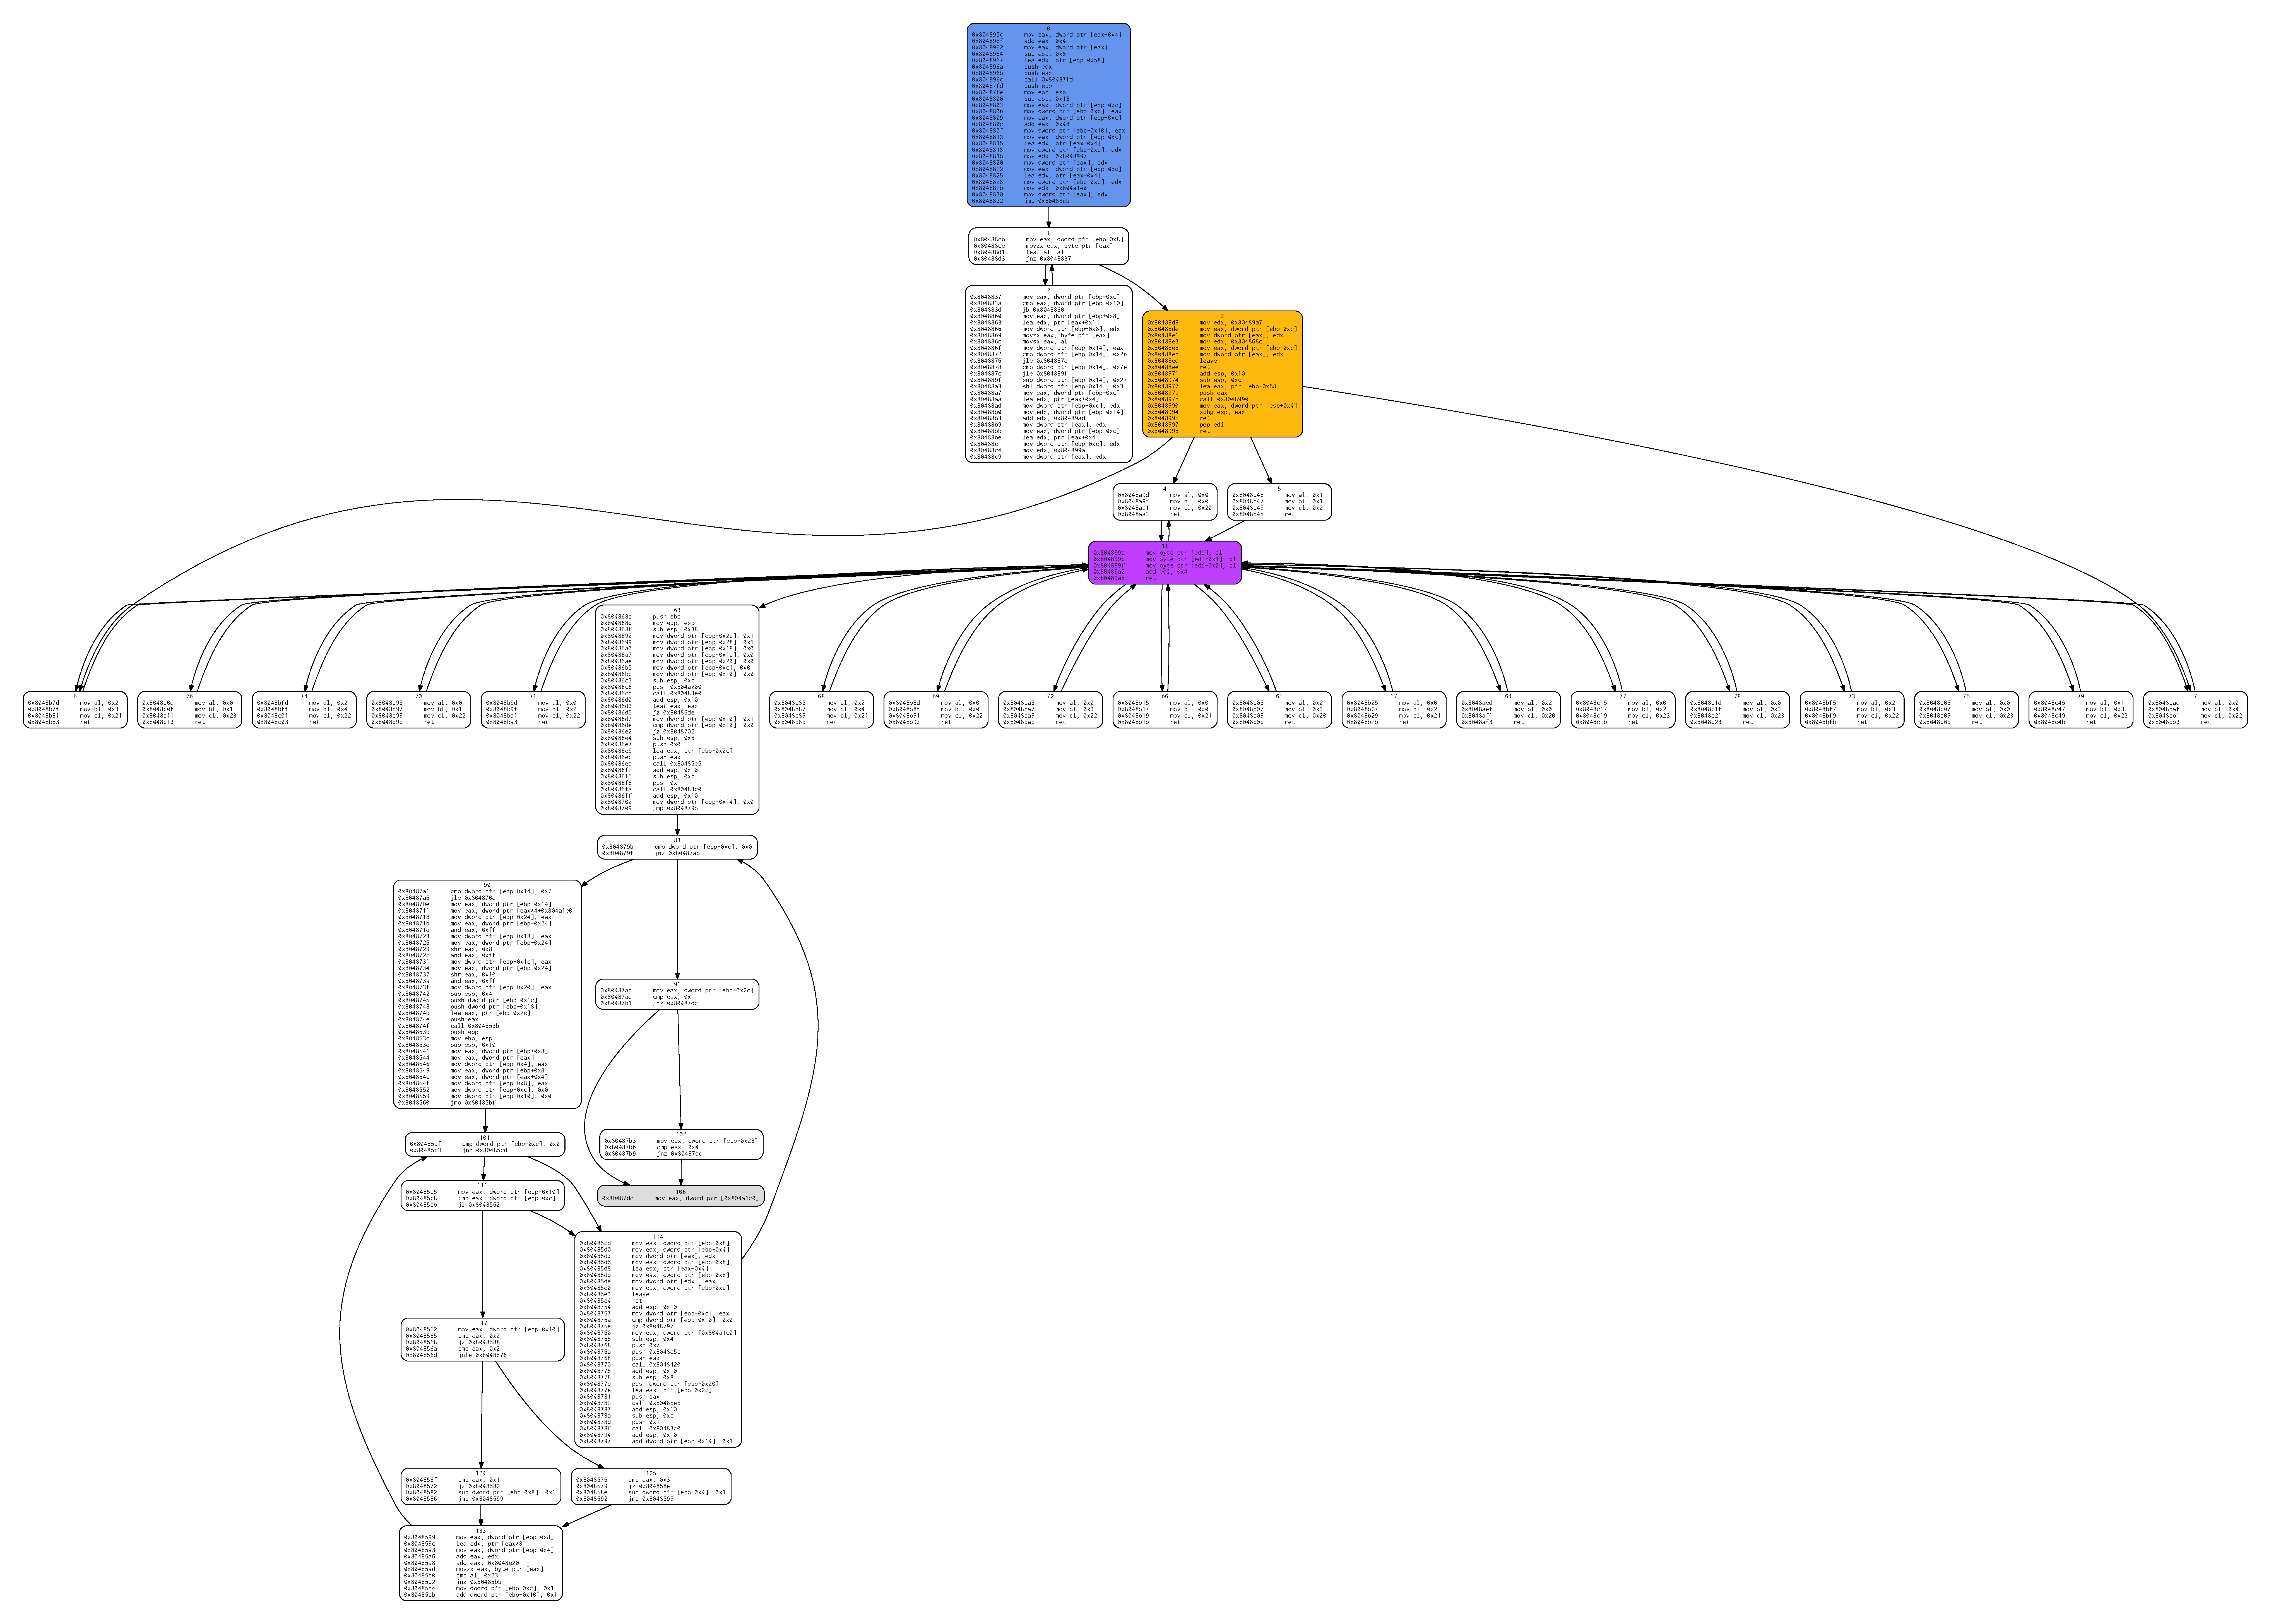
\includegraphics[width=0.8\textwidth,keepaspectratio]{mecung.pdf}
  \caption{Partial CFG}
  \label{fig:partial_cfg}
\end{figure}

\subsection{Other behavior analysis}
\label{sec:other_behavior_analysis}
No answer given in~\Cref{sec:static_analysis_quick} is solved, and even more questions are posed. We hopelessly observe the mazes shown by the challenge from different inputs, sometimes the star is displayed with different positions and locations, but nothing is clear.

\subsection{Failures and lessons learned}
When starting with challenge, I though that it must be resolved on interview time if not want to be rejected. I didn't focus on detail analyzing every machine instructions, I tried instead to figure out quickly its high level semantics though its behaviors; but this approach did not work in this case: the \emph{signal-to-noise} of observing the differences between printed out mazes is so small that I can only recognize the difference but cannot figure out any useful idea.
% I cannot resolve the challenge on the time of interview.

Samuel, the interviewer, has given generously tons of suggestions. After I have discovered quickly the existence of \texttt{SHOW\_ME\_THE\_MECUNG} but blocked (until the end of the interview) at understanding how the function at \texttt{0x804868c} relates with the input serial, he gave me the first hint (maybe he knows that I am Vietnamese):
\begin{quote}
  Sam: Hey, does ``me cung'' mean something in Vietnamese?\newline
  Me: Well, that means ``maze''.\newline
  Sam: This is a hint for you. 
\end{quote}
I do not quite understand what does it means, then I have tried naively some serials: \texttt{mecung}, \texttt{labyrinth}, \texttt{maze}, etc., but nothing works, obviously. 

Samuel noticed me the relation between the functions at \texttt{0x8048990} and at \texttt{0x80487fd}: they share indeed an argument. He then explained how the later can execute $3$-instructions code snippets by ``unrolling''  the stack organized by the former; but I could not grasp his suggestions to tackle the challenge :(.

% \paragraph{Lessons}
It should be better if we focus on the function at \texttt{0x80487fd} since the ``stack unrolling'' mechanism reveals the \emph{execution model} of the program, understanding this model is one of the keys to solve the challenge.

\section{Return-oriented programming}
\label{sec:detail_analysis}

In this section, we present a complete analysis which reveals the execution model of the challenge, then allows us to get a correct serial input. The analysis is done after the interview.

\subsection{Execution model}
\label{sec:execution_model}

As suggested by Samuel, the ``stack unrolling'' mechanism of the function at \texttt{0x80487fd} is a kind of \emph{object-oriented programming}~\autocite{shacham2007geometry} where each $3$-instructions (and a followed \texttt{ret}) code snippet is called a \emph{gadget}, some of them can be observed in~\Cref{fig:partial_cfg}. 
The execution model of the binary is realized by two function: one at \texttt{0x80487fd}, we named \texttt{execute\_rop\_table}; the other at \texttt{0x80487fd}, named \texttt{setup\_rop\_table}.

The function \texttt{execute\_rop\_table} transfers the control flow to the address contained in the first entry of a \emph{rop table} passed through its single argument. This address points to a gadget which ends with a \texttt{ret} instruction, that means it transfers the control flow to an address (of the next gadget) contained in the next $4$ bytes higher stack address. The semantics of \texttt{execute\_rop\_table} is presented by the \texttt{C++} function in~\Cref{lst:setup_rop_table}.

\begin{listing}[ht]
  \begin{tcolorbox}
\begin{minted}[tabsize=2]{c++}
auto execute_rop_table(size_t* rop_table) -> void
{
  using rop_fun = void(*)();
  auto entry_rop = reinterpret_cast<rop_fun>(rop_table[0]);
  return entry_rop();
}
\end{minted}
  \end{tcolorbox}
  \caption{\texttt{setup\_rop\_table}}
  \label{lst:setup_rop_table}
\end{listing}

\begin{remark}
  We note also that the rop table is located on the stack since the argument (i.e.~the address of the rop table) passed into \texttt{execute\_rop\_table} is also a local parameter of \texttt{main}.
\end{remark}

The \emph{rop table} is also the second argument of \texttt{setup\_rop\_table}, looking into this function (c.f.~\Cref{lst:setup_first_twos}) we observe that the first two entries of the rop table are fixed. Indeed, the first is \texttt{0x8048997} (c.f.~the \texttt{mov} instruction at \texttt{0x804881b}) which contains, beside the last \texttt{ret} instruction, only a \texttt{pop edi}. The second is a \emph{buffer} at \texttt{0x804a1e0} (c.f.~the \texttt{mov} instruction at \texttt{0x804882b}), this buffer is then moved into \texttt{edi} since the execution of the first gadget.

\begin{listing}
  \begin{minted}[frame=lines,tabsize=2]{nasm}
...
0x804881b      mov     edx, offset first_rop_entry
0x8048820      mov     [eax], edx
0x8048822      mov     eax, [ebp+current_rop]
0x8048825      lea     edx, [eax+4]
0x8048828      mov     [ebp+current_rop], edx
0x804882b      mov     edx, offset buffer
...
  \end{minted}
  \caption{Setup first two instructions}
  \label{lst:setup_first_twos}
\end{listing}

\paragraph{Abstract machine}
In summary, the binary has implemented actually by an \emph{abstract machine} whose opcodes are stored sequentially in the stack.
\begin{figure}[h]
  \centering
  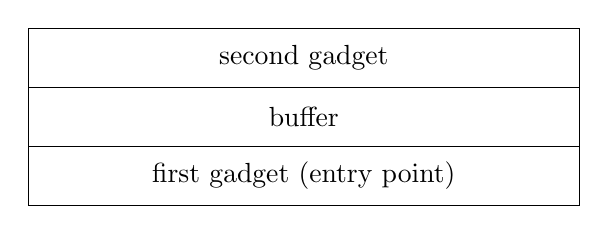
\begin{tikzpicture}
    \node[draw,align=center,minimum height=0.75cm,minimum width=7cm] (entry_point) at (0, 0) {first gadget (entry point)};
    \node[draw,align=center,minimum height=0.75cm,minimum width=7cm] (entry_point) at (0, 0.75) {buffer};
    \node[draw,align=center,minimum height=0.75cm,minimum width=7cm] (entry_point) at (0, 1.5) {second gadget};
  \end{tikzpicture}
  \caption{Execution model}
  \label{fig:execution_model}
\end{figure}

\printbibliography

\end{document}